\documentclass[11pt]{article}

\usepackage[utf8]{inputenc}
\usepackage[T1]{fontenc}
\usepackage[brazilian]{babel}
\usepackage[a4paper,margin=2.5cm]{geometry}
\usepackage{amsmath}
\usepackage{graphicx}
\usepackage{booktabs}
\usepackage{longtable}
\usepackage{caption}
\usepackage{float}
\usepackage{hyperref}

% Avoid leaving a single line of a paragraph alone at the top of the next page.
\widowpenalty=10000
\clubpenalty=10000

\title{Segmentação Automática de B-Lines em Ultrassom Pulmonar: \\
Comparação de Arquiteturas e Representações de Saída}
\author{}
\date{Outubro de 2026}

\begin{document}

\maketitle

% ============================================================
\section{Contexto e Objetivo}
% ============================================================

O projeto estuda a segmentação automática de B-Lines em ultrassom pulmonar. A ideia
central não é apenas treinar um modelo, mas montar uma estrutura de experimentos que
permita comparar arquiteturas diferentes usando o mesmo dataset e split, registrando
as diferenças de protocolo e aplicando métricas COCO comuns sempre que possível. A
pergunta central é como a representação e a supervisão geométrica afetam a
localização de B-Lines com poucas anotações.

As anotações originais estão no formato YOLO Polygon: cada B-Line é um quadrilátero
de 4 vértices (classe $x_1\ y_1\ x_2\ y_2\ x_3\ y_3\ x_4\ y_4$, coordenadas
normalizadas).

Em estudos de ultrassom pulmonar, a tarefa pode ser detecção, segmentação ou
localização do ponto de origem pleural; esses alvos não são intercambiáveis
\cite{lucassen2023}. Este trabalho avalia a localização da extensão anotada como
quadrilátero, sem inferir diagnóstico clínico.

\subsection{Trabalhos relacionados}

Há métodos específicos para B-Lines com alvos e protocolos diferentes. Lucassen et
al. estudam a localização do ponto de origem pleural, enquanto trabalhos recentes
exploram caixas poligonais para representar a forma da B-Line
\cite{lucassen2023,nabawanuka2025}. O LUS-BALD é um conjunto publicado com 401
imagens, partição por paciente e teste sem rótulos públicos \cite{lusbald2025}.
O conjunto local também soma 401 imagens, mas essa coincidência não comprova que
seja a mesma versão ou que preserve as partições publicadas; a proveniência ainda
precisa ser confirmada.

Como referências de parametrização e localização de quadriláteros, EAST e
TextBoxes++ predizem texto orientado, Gliding Vertex representa os vértices por
deslocamentos restritos em relação à caixa horizontal, e RoI Transformer aprende
transformações espaciais para alinhar regiões orientadas
\cite{zhou2017east,liao2018textboxes,xu2020gliding,ding2019roi}. CornerNet, por
sua vez, detecta caixas por pares de pontos-chave e aprende a associar os cantos
\cite{law2018cornernet}. Esses trabalhos motivam comparações de representação,
mas seus objetos e conjuntos de dados não são baselines numéricos diretamente
comparáveis aos deste projeto.

Uma loss Dice com informação de contorno já foi estudada em segmentação de
artefatos de ultrassom pulmonar \cite{abbasi2025}. O modelo, a saída e o conjunto
de dados desse trabalho diferem dos daqui; a referência motiva uma hipótese de
ablação, sem implicar equivalência à loss de IoU poligonal implementada aqui.

% ============================================================
\section{Dataset}
% ============================================================

O conjunto de treino tem 256 imagens. O conjunto de validação tem 75 imagens e 115
instâncias anotadas (1,53 B-Lines por imagem, em média). Existe ainda um conjunto de
teste com 70 imagens, mas sem rótulo até o momento.

Como o teste não tem anotação, todos os números reportados neste trabalho vêm do
conjunto de validação --- o mesmo usado para acompanhar o treino. Isso é discutido
na Seção~\ref{sec:limitacoes} como limitação.

A validação contém 75 arquivos de rótulo válidos e 115 instâncias, sem imagens
negativas. Na auditoria do treino, duas instâncias tinham cinco vértices, apesar de
o formato esperado ser um quadrilátero. Para tornar os loaders consistentes, ambas
foram convertidas para quatro vértices removendo o ponto cuja exclusão minimiza a
área do triângulo local. A correção e as linhas originais estão registradas em
\texttt{docs/annotation\_corrections.json}; essa aproximação altera uma das áreas
em 7,7\% e não confirma a intenção do anotador.

O repositório não registra a fonte original dos exames, identificadores de
paciente ou a regra usada para separar treino e validação. Portanto, não é possível
confirmar neste momento se imagens do mesmo paciente ficaram restritas a uma única
partição. Essa informação deve ser verificada antes de interpretar a validação como
independente. A licença, a autorização de uso e a situação de aprovação ética ou
isenção também não estão documentadas nos arquivos disponíveis e precisam ser
confirmadas antes de divulgação externa.

% ============================================================
\section{Protocolo Experimental}
% ============================================================

Mask R-CNN, Faster R-CNN e Polygon Head usam Detectron2 \cite{wu2019detectron2},
backbone ResNet-50 com FPN e inicializações do Model Zoo pré-treinadas no COCO
\cite{lin2014coco}. As configurações são
\texttt{mask\_rcnn\_R\_50\_FPN\_3x},
\texttt{faster\_rcnn\_R\_50\_FPN\_3x} e
\texttt{keypoint\_rcnn\_R\_50\_FPN\_3x}, respectivamente; a última recebe a
Polygon Head customizada. Os três usam batch de 4 imagens, taxa de aprendizado de
0,00025 e 2.000 iterações. A cada 100 iterações há avaliação e checkpoint. A seleção é
alinhada à tarefa: segm/AP para Mask R-CNN, bbox/AP para Faster R-CNN e
segm\_polygon/AP para Polygon Head. Um hook adicional calcula a loss de validação
sem augmentations aleatórias.

Os baselines e as quatro novas configurações poligonais foram executados com três
seeds (0, 1 e 2). Os resultados atuais são apresentados como média e desvio-padrão
amostral entre seeds. As diferenças entre framework, augmentations e hiperparâmetros
do YOLO permanecem como fatores de confusão na comparação entre famílias de modelos.

O YOLOv11n usa Ultralytics \cite{ultralytics2024}, pesos iniciais
\texttt{yolo11n.pt}, entrada de $640\times640$, batch de 16 e 31 épocas, nos mesmos
splits. O batch e a taxa de aprendizado seguem a configuração padrão desse
framework, e não foram igualados aos do Detectron2. As 31 épocas aproximam as
8.000 imagens vistas pelo protocolo Detectron2 ($2.000\times4$) para 256 imagens
de treino. As predições são convertidas para COCO e avaliadas com COCOeval
\cite{lin2014coco}; usar o mesmo avaliador não elimina as diferenças entre tarefas
e protocolos.

% ============================================================
\section{Mask R-CNN (baseline)}
\label{sec:maskrcnn}
% ============================================================

Arquitetura de referência do projeto \cite{he2017mask}: detecta a caixa
delimitadora do objeto e prevê uma máscara binária livre, pixel a pixel, para cada
instância.

Uma execução exploratória anterior mostrou sinais de overfitting: a loss de treino
cai continuamente até aproximadamente 0,28, mas a loss de validação para de melhorar
por volta da iteração 900--1400 (mínimo de 0,44) e volta a subir, chegando a 0,51 na
iteração final (Figura~\ref{fig:mask_loss}). Nessa mesma execução, o checkpoint
final não era o melhor: o AP de segmentação atingiu seu pico na iteração 1399
(40,61) e caiu para 38,33 na iteração 2000 (Figura~\ref{fig:mask_ap}). Por isso
passou-se a selecionar o melhor checkpoint em vez de sempre usar o último --- essa
mudança sozinha elevou o
AP de segmentação reportado de 36,7 para 40,6. Esses valores descrevem uma execução
anterior e não a média das três seeds da rodada atual, cujos resultados são
apresentados na tabela consolidada da Seção~\ref{sec:resumo}.

\begin{table}[H]
\centering
\caption{Mask R-CNN na rodada atual: média $\pm$ desvio-padrão amostral de três
seeds. A análise de loss e iteração descrita acima pertence à execução exploratória
anterior.}
\begin{tabular}{lccc}
\toprule
Saída & AP & AP50 & AP75 \\
\midrule
Caixa delimitadora (bbox) & $56,12\pm1,74$ & $91,23\pm2,01$ & $59,89\pm4,13$ \\
Segmentação (segm) & $42,88\pm0,70$ & $86,14\pm0,98$ & $35,98\pm1,09$ \\
\bottomrule
\end{tabular}
\end{table}

Na rodada atual, a avaliação por instância de máscara, com matching um-para-um e
IoU $\geq0{,}50$, obteve precisão de $79,01\pm5,83\%$, recall de
$88,99\pm4,79\%$ e F1 de $83,47\pm1,15\%$. O limiar que maximiza F1 na validação
foi $0,67\pm0,10$. A execução exploratória anterior reportou outros valores de
IoU/Dice e threshold; eles não são agregados comparáveis à métrica da rodada atual.
Naquela análise anterior, foram registrados IoU médio 0,52 (mediana 0,65), Dice
médio 0,61 (mediana 0,78), precisão 0,59, recall 0,67 e confiança média 0,91. No
threshold anterior de 0,875, o F1 reportado foi 0,82 (precisão 0,81, recall 0,83).

Vale registrar que, ao inspecionar as máscaras visualmente com o threshold padrão
(0,50), apareciam máscaras borradas e detecções extras (2,31 por imagem, contra
1,53 reais). Usando o threshold ótimo do próprio modelo, esse problema quase
desapareceu --- parte do que parecia ``modelo ruim'' era, na verdade, visualização
calibrada de forma inadequada.

\begin{figure}[H]
\centering
\includegraphics[width=0.8\linewidth]{figures/mask_rcnn/train_vs_val_loss.png}
\caption{Loss de treino vs.\ validação ao longo das 2000 iterações. A validação
para de melhorar por volta da iteração 1000 e volta a subir no final.}
\label{fig:mask_loss}
\end{figure}

\begin{figure}[H]
\centering
\includegraphics[width=0.8\linewidth]{figures/mask_rcnn/val_segm_ap.png}
\caption{AP de segmentação de validação ao longo do treino. O pico ocorre antes da
iteração final.}
\label{fig:mask_ap}
\end{figure}

\begin{figure}[H]
\centering
\includegraphics[width=0.8\linewidth]{figures/mask_rcnn/coco_pr_curves.png}
\caption{Curva precisão--recall do COCOeval para a segmentação. O eixo horizontal
é recall e o vertical é precisão. As curvas mostram os limiares de IoU 0,50 e
0,75; a curva tracejada representa a média dos limiares de IoU entre 0,50 e 0,95.}
\label{fig:mask_pr}
\end{figure}

\begin{figure}[H]
\centering
\includegraphics[width=0.6\linewidth]{figures/predictions/mask_rcnn_1646467410642.png}
\caption{Exemplo de predição (verde: anotação real; vermelho: máscara prevista).}
\label{fig:mask_pred}
\end{figure}

\begin{figure}[H]
\centering
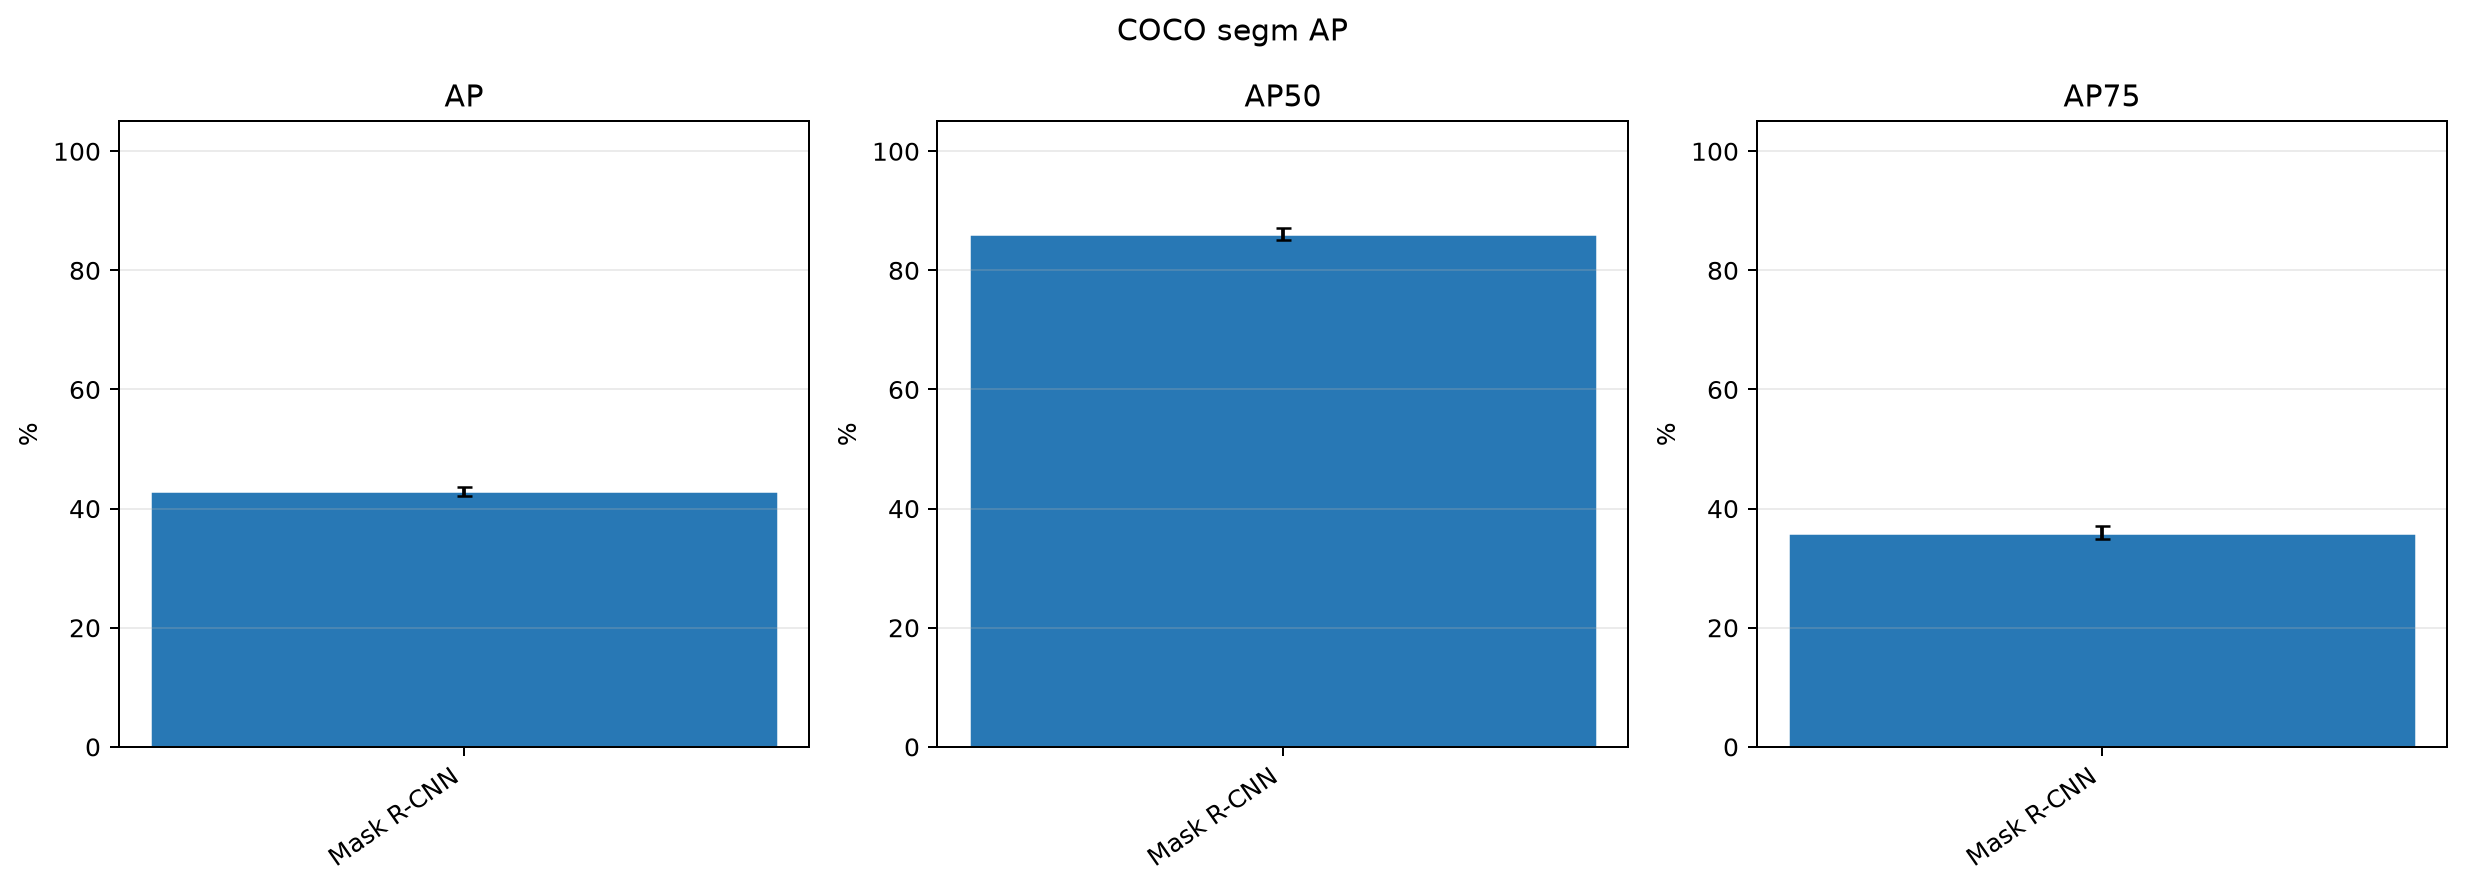
\includegraphics[width=0.8\linewidth]{reports/coco_ap_segm.png}
\caption{AP de segmentação por máscara do Mask R-CNN na rodada atual.}
\label{fig:mask_ap_current}
\end{figure}

% ============================================================
\section{Faster R-CNN}
% ============================================================

Faster R-CNN \cite{ren2015faster} compartilha a família de detectores por regiões,
mas não prevê máscaras: detecta apenas a caixa delimitadora. O objetivo foi isolar
a dificuldade de localizar a B-Line da dificuldade de desenhar sua forma exata.
Utiliza o mesmo dataset já registrado, sem uma conversão de arquivos separada; o
loader deriva a caixa delimitadora a partir dos vértices poligonais.

\begin{table}[H]
\centering
\caption{Faster R-CNN na rodada atual: média $\pm$ desvio-padrão amostral de
três seeds.}
\begin{tabular}{lccc}
\toprule
AP & AP50 & AP75 & P/R/F1 (IoU 0,50) \\
\midrule
$52,37\pm2,38$ & $87,95\pm1,72$ & $55,05\pm4,23$ &
$82,96\pm1,85 / 85,80\pm1,33 / 84,33\pm0,41$ \\
\bottomrule
\end{tabular}
\end{table}

O limiar de confiança que maximiza F1 na validação foi $0,74\pm0,08$. Na execução
anterior havia sido reportado F1 0,85 com limiar 0,53; os números novos usam três
seeds e matching/seleção de threshold padronizados nesta rodada.

\begin{figure}[H]
\centering
\includegraphics[width=0.6\linewidth]{figures/predictions/faster_rcnn_1646467410642.png}
\caption{Exemplo de predição do Faster R-CNN (verde: anotação real; vermelho: caixa
prevista).}
\label{fig:faster_pred}
\end{figure}

\begin{figure}[H]
\centering
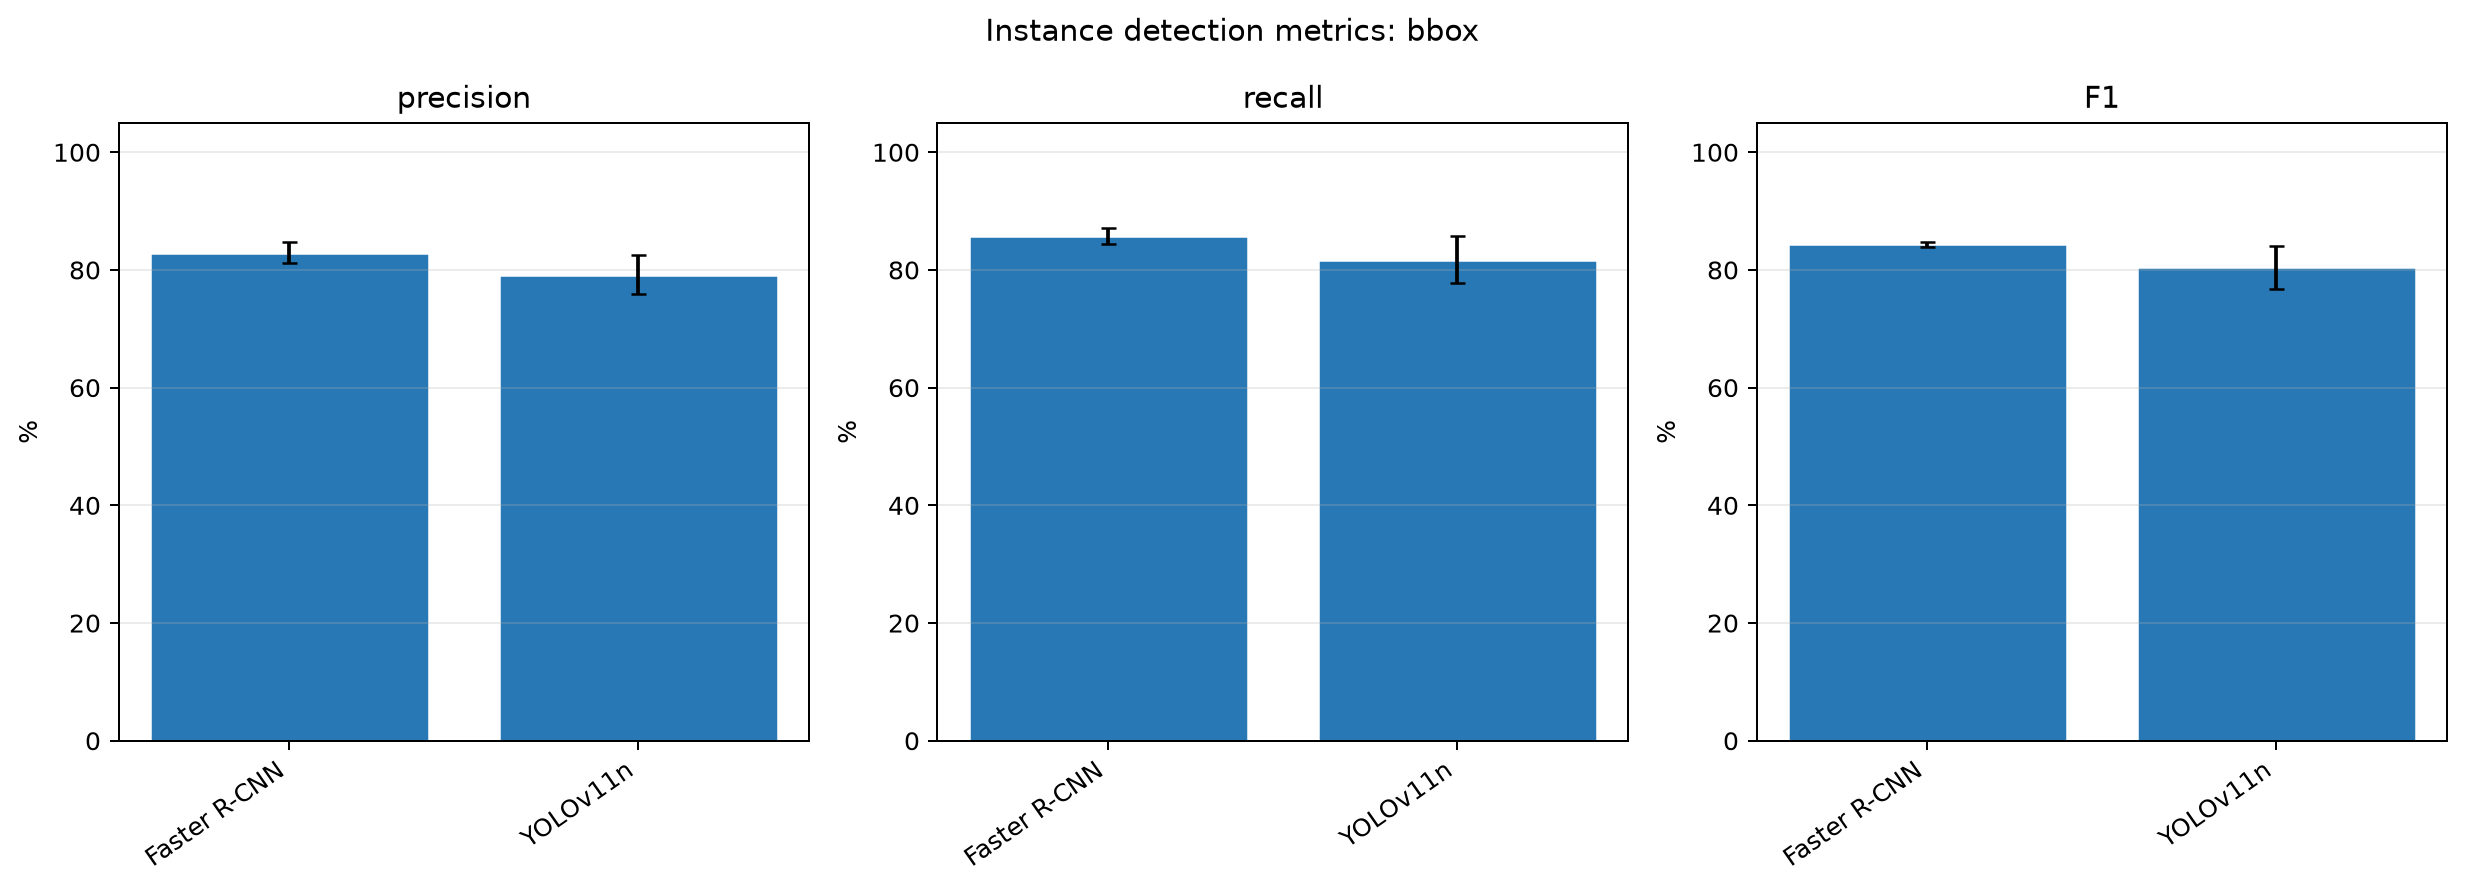
\includegraphics[width=0.8\linewidth]{reports/detection_metrics_bbox.png}
\caption{Precisão, recall e F1 por instância para os detectores de caixa na
rodada atual.}
\label{fig:bbox_metrics}
\end{figure}

% ============================================================
\section{YOLOv11}
% ============================================================

Arquitetura \textit{one-stage}, de família diferente da R-CNN (Ultralytics), usada
para verificar se a dificuldade observada era específica dos modelos R-CNN.
Utilizou-se o \texttt{yolo11n} (variante nano), com o dataset convertido de
polígono para caixa a partir da mesma anotação original, treinado por 31 épocas ---
equivalente ao número de imagens vistas pelo protocolo dos R-CNN (2000 iterações
$\times$ 4 de batch / 256 imagens). Os hiperparâmetros de treino seguiram os padrões
do Ultralytics; não foram forçados os mesmos valores do Detectron2, pois transportar
hiperparâmetros de um framework para outro tende a prejudicar a convergência.

As predições foram exportadas para o formato COCO e avaliadas com o mesmo código
\texttt{pycocotools} utilizado nos demais modelos, não com a métrica nativa do
Ultralytics, para padronizar o avaliador na tarefa de caixas. Isso não torna os
protocolos de treinamento idênticos.

\begin{table}[H]
\centering
\caption{YOLOv11n na rodada atual: média $\pm$ desvio-padrão amostral de três
seeds.}
\begin{tabular}{lccc}
\toprule
AP & AP50 & AP75 & P/R/F1 (IoU 0,50) \\
\midrule
$55,86\pm0,99$ & $85,26\pm2,14$ & $59,39\pm2,66$ &
$79,20\pm3,32 / 81,74\pm3,98 / 80,45\pm3,63$ \\
\bottomrule
\end{tabular}
\end{table}

O limiar de confiança médio escolhido na validação foi $0,38\pm0,04$. A execução
anterior reportava F1 0,82 com limiar 0,53; esse valor foi substituído pela
avaliação de três seeds mostrada acima.

\begin{figure}[H]
\centering
\includegraphics[width=0.6\linewidth]{figures/predictions/yolo_1646467410642.png}
\caption{Exemplo de predição do YOLOv11 (verde: anotação real; vermelho: caixa
prevista).}
\label{fig:yolo_pred}
\end{figure}

% ============================================================
\section{Comparação entre os Três Modelos de Caixa}
% ============================================================

\begin{table}[H]
\centering
\caption{Comparação atual de AP de caixa entre Mask R-CNN, Faster R-CNN e
YOLOv11n (média $\pm$ desvio-padrão de três seeds).}
\begin{tabular}{lccc}
\toprule
Modelo & AP & AP50 & AP75 \\
\midrule
Mask R-CNN (caixa) & $56,12\pm1,74$ & $91,23\pm2,01$ & $59,89\pm4,13$ \\
Faster R-CNN & $52,37\pm2,38$ & $87,95\pm1,72$ & $55,05\pm4,23$ \\
YOLOv11n & $55,86\pm0,99$ & $85,26\pm2,14$ & $59,39\pm2,66$ \\
\bottomrule
\end{tabular}
\end{table}

Na rodada atual, o AP de caixa varia de $52,37\%$ (Faster R-CNN) a $56,12\%$
(Mask R-CNN); YOLOv11n obteve $55,86\%$. A diferença entre as médias é descritiva,
e a variação entre seeds deve ser considerada. As arquiteturas usam protocolos de
treino parcialmente diferentes.

\begin{figure}[H]
\centering
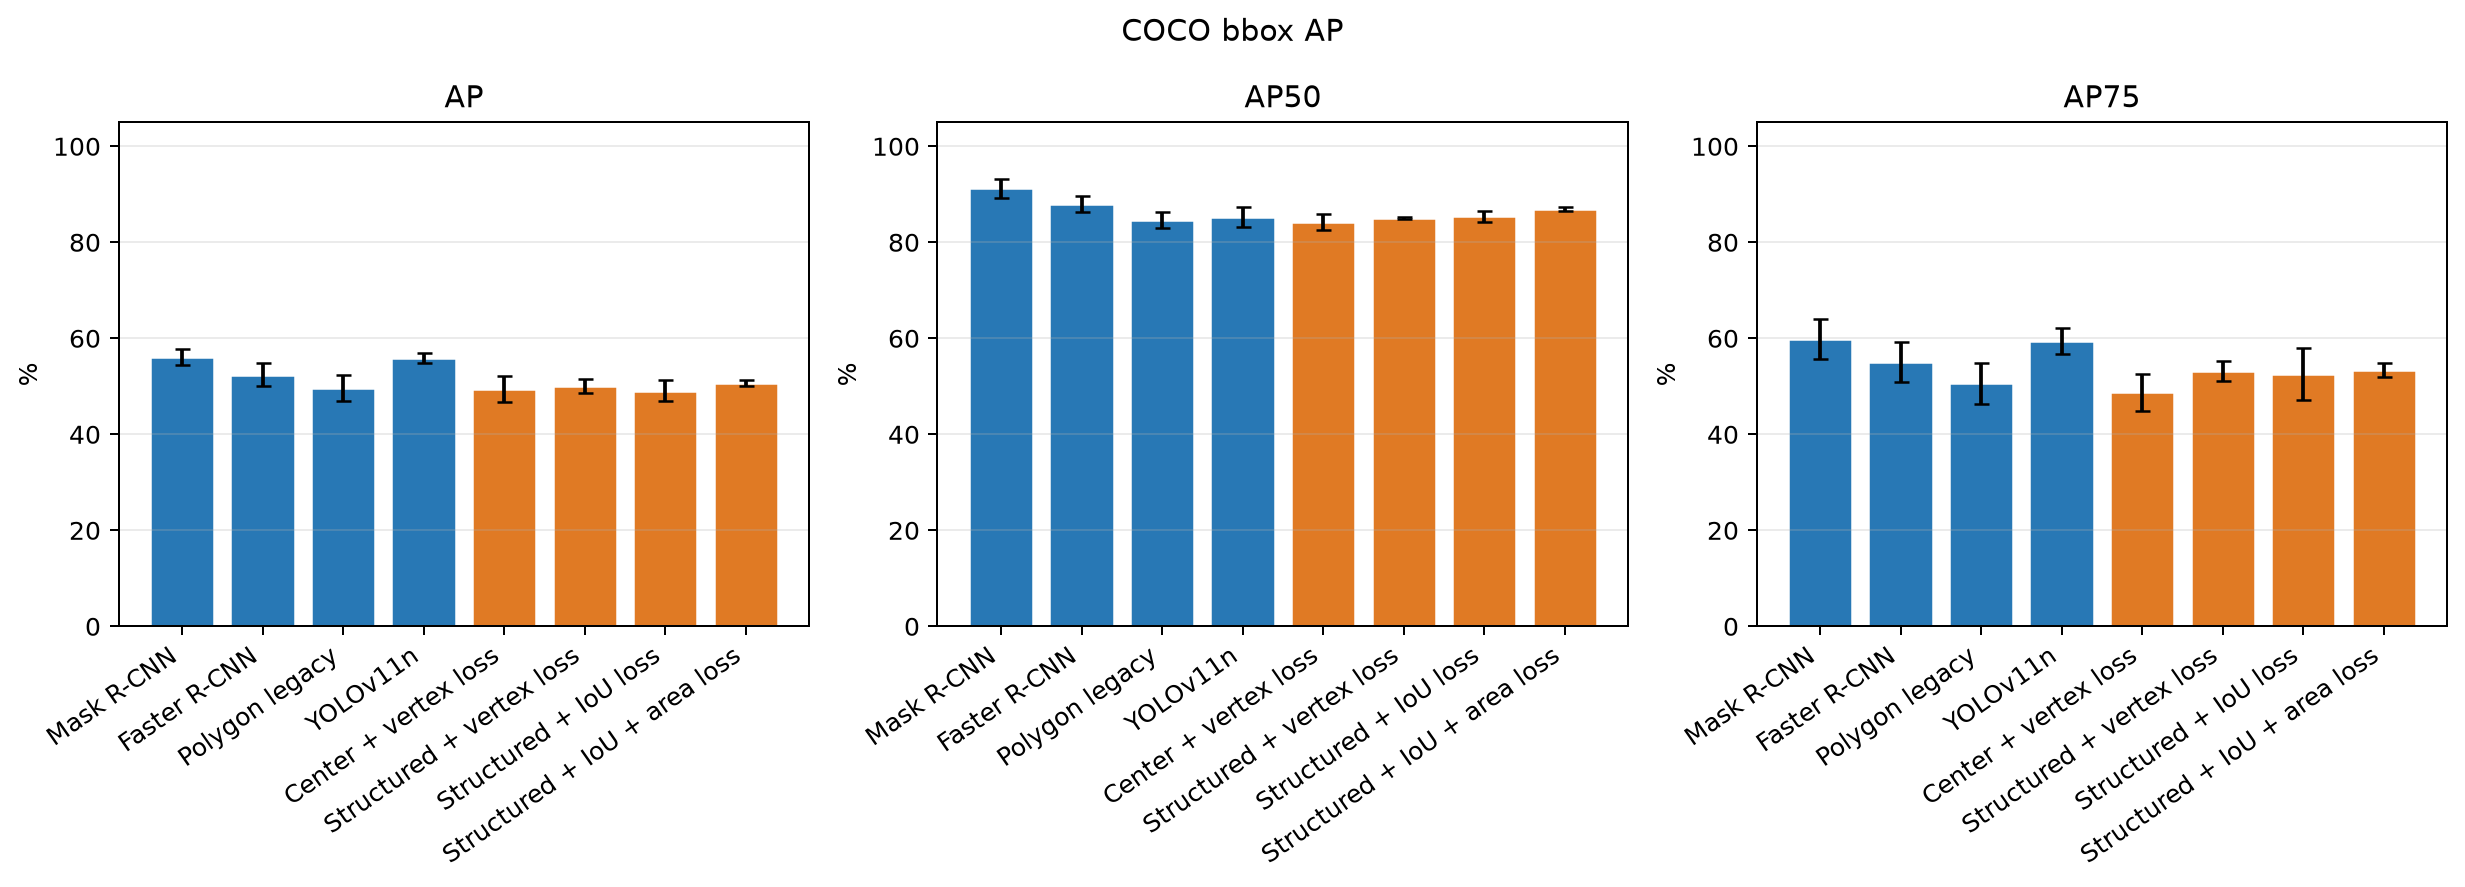
\includegraphics[width=0.7\linewidth]{reports/coco_ap_bbox.png}
\caption{Comparação atual de AP/AP50/AP75 para os detectores de caixa.}
\label{fig:comparison}
\end{figure}

% ============================================================
\section{Polygon Head --- Primeira Tentativa (Heatmap)}
% ============================================================

Em vez de uma máscara livre, a proposta da Polygon Head é prever diretamente os 4
vértices do quadrilátero. Na primeira tentativa, reaproveitou-se a infraestrutura
de Keypoint R-CNN já disponível no Detectron2 (originalmente concebida para pose
humana, com 17 pontos), adaptada para 4 pontos --- cada vértice tratado como um
ponto-chave localizado por um mapa de calor espacial. A opção por reaproveitar essa
infraestrutura, em vez de implementar algo do zero, teve como objetivo evitar
reimplementar, sem GPU disponível para testes interativos, as partes mais
arriscadas: a transformação correta dos pontos quando a imagem sofre corte ou
espelhamento durante o treino.

\begin{table}[H]
\centering
\caption{Resultados exploratórios de execução única da Polygon Head heatmap,
preservados como registro das primeiras tentativas.}
\begin{tabular}{lccccc}
\toprule
Configuração & AP & AP50 & AP75 & Melhor F1 (\%) & \% polígono inválido \\
\midrule
Resolução padrão & 15,0 & 37,1 & 11,9 & 49 & 6,7\% \\
Resolução dobrada & 3,8 & 10,8 & 2,7 & 25 & 20,4\% \\
\bottomrule
\end{tabular}
\end{table}

\noindent \textit{Polígono inválido}: os 4 vértices, conectados na ordem prevista,
formam uma figura que se autointersecciona --- não é um quadrilátero simples.

Aumentar a resolução do mapa de calor piorou o resultado em vez de melhorá-lo. Com
poucos dados (256 imagens) e poucas iterações, um alvo de classificação mais fino
é mais difícil de aprender, não mais fácil. Além disso, o heatmap trata os 4
vértices como classificações independentes entre si --- nada na arquitetura obriga
os pontos a formarem uma figura geometricamente coerente, o que explica a taxa de
autointersecção observada.

Para permitir comparação pelo mesmo avaliador, o polígono previsto foi convertido
em uma região preenchida e avaliado pelo COCOeval de segmentação, com a métrica
denominada \texttt{segm\_polygon}. O avaliador é comum, mas a saída geométrica não
é idêntica à máscara livre do Mask R-CNN; essa distinção é mantida nas
interpretações.

% ============================================================
\section{Polygon Head --- Regressão Direta de Vértice}
% ============================================================

Diante do diagnóstico de que o problema estava no paradigma de classificação por
mapa de calor, a alternativa foi prever diretamente as coordenadas $(x, y)$ de cada
vértice --- regressão contínua em vez de classificação em grade. Como essa opção
não existe pronta no Detectron2, foi implementada uma cabeça de rede nova: quatro
camadas convolucionais, um \textit{pooling} global e duas camadas densas,
terminando em 8 números (4 vértices $\times$ 2 coordenadas) por objeto detectado. A
função de perda é \textit{smooth-L1}, comparando a posição prevista com a real,
ambas normalizadas em relação à própria caixa do objeto --- a mesma técnica já
utilizada pela regressão de \textit{bounding box} do Detectron2.

\begin{table}[H]
\centering
\caption{A configuração sem restrição foi reexecutada na rodada de três seeds; os
resultados de sigmoid e penalidade são os registros das primeiras execuções.}
\begin{tabular}{lccccc}
\toprule
Configuração & AP & AP50 & AP75 & F1 (\%) & Recall@0,5 (\%) \\
\midrule
Sem restrição (legacy, atual) & $14,36\pm0,73$ & $52,86\pm0,70$ & $1,63\pm0,44$ & $60,36\pm2,35$ & $58,84\pm4,46$ \\
Com sigmoid na saída (inicial) & 4,3 & 22,9 & 0,1 & 37 & 42 \\
Com penalidade suave (inicial) & 8,2 & 35,3 & 0,1 & 46 & 55 \\
\bottomrule
\end{tabular}
\end{table}

O limiar médio de confiança selecionado para a configuração legacy atual foi
$0,866\pm0,002$. A primeira execução sem restrição, antes da repetição, tinha AP
12,2, AP50 54,2 e AP75 1,4; a nova linha da tabela substitui esses valores como
resultado principal da configuração reexecutada, sem apagar o registro inicial
descrito abaixo.

Nas três execuções exploratórias iniciais de regressão direta (sem restrição,
sigmoid e penalidade), o relatório da época registrou 0\% de polígonos
autointersectados, em comparação com 6,7--20,4\% nas execuções de heatmap. Esse
resultado histórico não foi recalculado para as três seeds atuais; portanto, não
estabelece que a nova rodada tenha taxa zero nem que a regressão direta elimine
sempre esse tipo de erro.

Na primeira execução da versão sem restrição (AP 12,2; AP50 54,2; AP75 1,4),
apesar de superior às duas correções então testadas, os polígonos eram cerca de
20\% maiores que o real, e 88\% das predições apresentavam algum vértice fora da
própria caixa prevista, já que nada na arquitetura impedia isso. Duas correções
foram testadas. A primeira, uma função sigmoide forçando a saída entre 0 e 1,
piorou o resultado: os alvos reais concentram-se exatamente nos valores extremos
(0 e 1, pois a caixa é definida pelos próprios vértices), e é justamente nesse
ponto que o gradiente da sigmoide é menor --- o efeito foi travar o aprendizado em
vez de apenas limitar a saída. A segunda, uma penalidade suave que atua somente
quando o vértice ultrapassa o intervalo válido, também piorou o resultado, e de
forma reveladora: a taxa de vértices fora da caixa não se alterou (permaneceu em
torno de 88\%), evidenciando que esse comportamento nunca foi a causa do problema,
apenas um sintoma correlacionado.

Uma análise exploratória anterior sugeriu caixas previstas 12--16\% maiores que as
anotadas. Esse valor ainda não foi confirmado quantitativamente nas predições da
rodada atual nem pode ser atribuído a todos os detectores. Como os vértices são
parametrizados em relação à proposta, um viés na caixa pode propagar-se para a
geometria; a rotina de análise de viés foi implementada e deve ser executada antes
de tratar essa hipótese como causa estabelecida.

\begin{figure}[H]
\centering
\includegraphics[width=0.6\linewidth]{figures/predictions/polygon_head_1646467410642.png}
\caption{Exemplo de predição da Polygon Head, regressão direta (verde: anotação
real; vermelho: polígono previsto).}
\label{fig:polygon_pred}
\end{figure}

% ============================================================
\section{Polygon Head --- Representação Estruturada e Losses Geométricas}
\label{sec:polygon_ablation}
% ============================================================

Depois das tentativas iniciais com heatmaps e regressão direta, foi implementada
uma nova rodada controlada de ablações. O objetivo foi testar parametrizações e
supervisões geométricas específicas para B-lines, mantendo o dataset, as propostas
e o protocolo Detectron2. Cada configuração foi executada com três seeds.

A configuração \textit{center-relative} representa os quatro vértices como offsets
ao centro da proposta. Ela ainda prevê oito valores por região: quatro pares
$(\Delta x_i,\Delta y_i)$, um para cada vértice. Na representação
\textit{structured}, a cabeça prevê sete parâmetros geométricos, dos quais os
quatro vértices são reconstruídos. Portanto, os valores 6 e 7 são as larguras das
duas extremidades do quadrilátero, não medidas separadas para cada vértice.

O fluxo de predição é o seguinte. A imagem passa pela rede convolucional e pela
FPN; o detector de regiões (RPN) propõe caixas; os recursos dentro de cada caixa
passam pela cabeça de regiões (RoI head). Para cada região candidata, a cabeça de
polígono produz os sete valores abaixo. A classe e a confiança determinam quais
regiões são mantidas na inferência, e os parâmetros geométricos de cada região
mantida são decodificados em quatro pontos $(x,y)$ na imagem.

Seja a caixa proposta $B=(x_0,y_0,x_1,y_1)$, com largura $w_B=x_1-x_0$,
altura $h_B=y_1-y_0$, diagonal $D=\sqrt{w_B^2+h_B^2}$ e centro
$c_B=((x_0+x_1)/2,(y_0+y_1)/2)$. A saída estruturada é
\[
\mathbf{q}=(q_1,\ldots,q_7)
= (\delta_x,\delta_y,c_2,s_2,\ell,a_-,a_+).
\]
Os dois primeiros valores posicionam o centro do polígono em relação ao centro
da proposta; $(c_2,s_2)$ codifica a orientação; $\ell$ codifica o comprimento;
e $a_-$ e $a_+$ codificam as larguras nas extremidades negativa e positiva do
eixo principal. A decodificação é:
\[
\begin{aligned}
 c &= c_B+(\delta_x w_B,\delta_y h_B), &
 \theta &= \tfrac12\operatorname{atan2}(s_2,c_2),\\
 L &= D\exp(\ell), &
 W_- &= D\exp(a_-),\quad W_+=D\exp(a_+),\\
 u&=(\cos\theta,\sin\theta), & v&=(-\sin\theta,\cos\theta),\\
 c_-&=c-\tfrac{L}{2}u, & c_+&=c+\tfrac{L}{2}u.
\end{aligned}
\]
Os vértices, na ordem usada pela implementação, são
\[
v_1=c_- -\tfrac{W_-}{2}v,\quad
v_2=c_+ -\tfrac{W_+}{2}v,\quad
v_3=c_+ +\tfrac{W_+}{2}v,\quad
v_4=c_- +\tfrac{W_-}{2}v.
\]
O uso de $(\cos2\theta,\sin2\theta)$ representa a orientação de um eixo sem
introduzir uma descontinuidade quando o mesmo eixo é descrito por ângulos que
diferem em $\pi$. Os parâmetros de comprimento e largura são logaritmos de
razões em relação a $D$; a exponencial recupera medidas positivas em pixels.

\begin{table}[H]
\centering
\caption{Interpretação dos sete valores previstos pela cabeça estruturada.}
\small
\begin{tabular}{clp{8.2cm}}
\toprule
Saída & Exemplo numérico & Significado e decodificação \\
\midrule
1--2 & $0,\ 0$ & Deslocamento do centro: o centro previsto coincide com o centro da caixa proposta. \\
3--4 & $1,\ 0$ & $(\cos2\theta,\sin2\theta)=(1,0)$, portanto $\theta=0$; o eixo longo fica horizontal. \\
5 & $\ln(0,5)\approx-0,693$ & Comprimento $L=0,5D$. Para $D=141,42$ px, $L=70,71$ px. \\
6 & $\ln(0,2)\approx-1,609$ & Largura da extremidade negativa: $W_-=0,2D=28,28$ px. \\
7 & $\ln(0,1)\approx-2,303$ & Largura da extremidade positiva: $W_+=0,1D=14,14$ px. \\
\bottomrule
\end{tabular}
\end{table}

Por exemplo, para a caixa $B=(100,50,200,150)$ px, o centro é $(150,100)$ px,
$w_B=h_B=100$ px e $D=141,42$ px. A saída
$(0,0,1,0,-0,693,-1,609,-2,303)$ produz aproximadamente os vértices
$(115,86)$, $(185,93)$, $(185,107)$ e $(115,114)$ px. Assim, a previsão não
estima “comprimento e largura de cada vértice”: estima centro, eixo, comprimento
e duas larguras de extremidade, e uma transformação determinística calcula os
quatro vértices. O quadrilátero resultante tem lados longos paralelos, isto é, a
representação impõe uma família geométrica mais restrita que quatro pontos livres.

Foram comparadas quatro variantes novas: centro relativo com vertex loss;
geometria estruturada com vertex loss; geometria estruturada com vertex loss mais
IoU poligonal suave; e a última configuração acrescida de loss relativa de área.
A variante legacy com vertex loss também foi reexecutada como referência nas
baselines. Em todas, a \textit{vertex loss} é a Smooth L1 entre os valores
previstos e os valores-alvo codificados na representação escolhida. Nas variantes
com IoU, soma-se a essa loss uma penalidade de sobreposição poligonal suave,
aproximada por rasterização diferenciável numa grade $32\times32$. Na variante
final, soma-se também o erro relativo entre as áreas previstas e anotadas. Em
notação resumida, a loss total é
\[
\mathcal{L}=\mathcal{L}_{\mathrm{vertex}}
+0{,}1\,\mathcal{L}_{\mathrm{IoU\ suave}}
+0{,}1\,\frac{|A_{\mathrm{pred}}-A_{\mathrm{gt}}|}{A_{\mathrm{gt}}},
\]
omitindo-se os termos de IoU e área nas variantes que não os usam. A IoU suave é
uma aproximação para treinamento; a avaliação reportada continua sendo feita pelo
COCOeval sobre os polígonos reconstruídos.

\subsection{O que a loss de IoU mede e por que acrescentar área?}

A IoU entre duas regiões é a razão entre a área de interseção e a área de união,
\[
\operatorname{IoU}(P,G)=\frac{|P\cap G|}{|P\cup G|}.
\]
Para polígonos, uma forma exata de treinamento exigiria calcular interseções e
uniões com operações geométricas que não são diferenciáveis em todos os casos.
Por isso, a implementação usa uma aproximação diferenciável. Ela amostra uma
grade $32\times32$ na região normalizada da proposta e, para cada ponto da grade,
estima suavemente se o ponto está dentro do quadrilátero. Para um polígono convexo,
a ocupação é obtida combinando as distâncias assinadas às quatro arestas por
sigmoides. Se $p_i$ e $g_i$ são as ocupações suaves previstas e anotadas no ponto
$i$, respectivamente, a aproximação é
\[
\operatorname{IoU}_{\mathrm{suave}}(P,G)=
\frac{\sum_i p_i g_i}{\sum_i (p_i+g_i-p_i g_i)},\qquad
\mathcal{L}_{\mathrm{IoU}}=1-\operatorname{IoU}_{\mathrm{suave}}.
\]
O alvo é mantido fixo durante a diferenciação; o gradiente orienta a previsão a
aumentar a sobreposição e reduzir a região prevista fora do alvo. Esta rasterização
suave é apenas uma surrogate de treino. Ela não é a IoU exata nem a métrica
reportada: na avaliação, COCOeval calcula a IoU dos polígonos previstos e anotados
com seu procedimento de segmentação.

A IoU já depende da interseção e das áreas dos dois polígonos; portanto, a loss de
área não acrescenta uma informação geométrica independente. Ela dá peso explícito
à diferença relativa de escala,
\[
\mathcal{L}_{\mathrm{área}}=
\frac{|A_{\mathrm{pred}}-A_{\mathrm{gt}}|}{A_{\mathrm{gt}}},
\]
e pode complementar a aproximação rasterizada, cuja resolução finita pode tornar
menos direto o sinal de correção para polígonos muito estreitos ou com escala
incorreta. Essa é uma justificativa plausível, não uma causa demonstrada pelos
experimentos. Na ablação observada, adicionar área à configuração estruturada com
IoU elevou o AP de $17,82\%$ para $20,15\%$, o AP50 de $57,92\%$ para $60,08\%$ e
o F1 de $63,64\%$ para $65,83\%$; porém, o AP75 caiu de $5,87\%$ para $5,26\%$.
Logo, o ganho foi descritivo e não ocorreu em todas as métricas. Com três seeds e
uma validação pequena, não se pode concluir que a loss de área seja a causa do
ganho nem que ele seja estatisticamente significativo.

\subsection{Ordem dos vértices, correspondência e validade geométrica}

Na regressão direta legacy, a Smooth L1 compara cada coordenada prevista com a
coordenada do mesmo índice no alvo. Uma permutação dos quatro vértices, mesmo que
descreva visualmente o mesmo quadrilátero, pode produzir uma loss grande. Para
reduzir esse problema, o loader ordena os pontos do alvo angularmente em torno do
centroide e escolhe como início o ponto mais alto; o mapper repete a ordenação
depois das transformações geométricas. Assim, as coordenadas supervisionadas têm
uma ordem cíclica consistente. Ainda assim, a regressão direta pode prever pontos
que se cruzam: a ordenação do alvo não impõe validade às previsões.

Na representação estruturada, a codificação do alvo usa o conjunto geométrico dos
quatro pontos para calcular centroide, eixo principal, comprimento e larguras; não
faz pareamento de $v_1$ previsto com $v_1$ anotado. A orientação usa
$(\cos 2\theta,\sin 2\theta)$, de modo que a direção do mesmo eixo não muda ao
trocar o sentido do vetor principal. A Smooth L1 compara esses parâmetros
geométricos. Além disso, o decodificador constrói os quatro vértices em ordem
cíclica ao redor do trapézio, com comprimento e larguras positivos. Isso impede a
autointerseção causada por uma simples inversão dos vértices na saída. As perdas
suaves de IoU e área operam sobre a forma reconstruída, sem comparar índices de
vértices individualmente. A rasterização da IoU, contudo, percorre as arestas do
alvo; por isso, os vértices anotados ainda precisam estar em ordem cíclica. O
loader e o mapper impõem essa ordem antes do cálculo da loss.

Essa propriedade depende da hipótese de que a anotação representa um quadrilátero
convexo, coerente com o formato trapezoidal imposto. A codificação do eixo
principal pode ser instável para formas quase simétricas ou degeneradas; a
representação estruturada também não consegue reproduzir quadriláteros arbitrários
fora de sua família geométrica. Portanto, ela reduz ambiguidades de ordem e
autointerseção, mas não torna toda anotação ou previsão automaticamente correta.

Se a saída for alterada para uma máscara, a comparação natural é entre mapas de
ocupação pixel a pixel, por exemplo com Dice ou IoU de máscara. Nesse caso, a ordem
dos vértices deixa de ser relevante para a loss da máscara; uma ordenação canônica
continua necessária apenas se a rede ainda supervisionar pontos-chave explicitamente.

Na rodada atual, a geometria estruturada com vertex loss elevou o AP poligonal
médio de $14,36\%$ (legacy) para $18,57\%$. Adicionar somente IoU suave resultou
em AP médio de $17,82\%$, mas o AP75 subiu de $2,08\%$ para $5,87\%$. A
configuração com IoU e área alcançou o maior AP poligonal ($20,15\%$), AP50
($60,08\%$) e F1 por instância ($65,83\%$). O AP75 permaneceu baixo
($5,26\%$), indicando que a localização precisa ainda é difícil. As diferenças
são descritivas; três seeds e 75 imagens não bastam para afirmar significância
estatística.

A tabela~\ref{tab:resumo_comparativo} reúne os resultados antigos preservados e
os valores atuais. Os valores das primeiras tentativas permanecem identificados
como execução única; eles não foram reexecutados na nova matriz e seus limiares e
protocolos podem diferir dos atuais.

\begin{figure}[H]
\centering
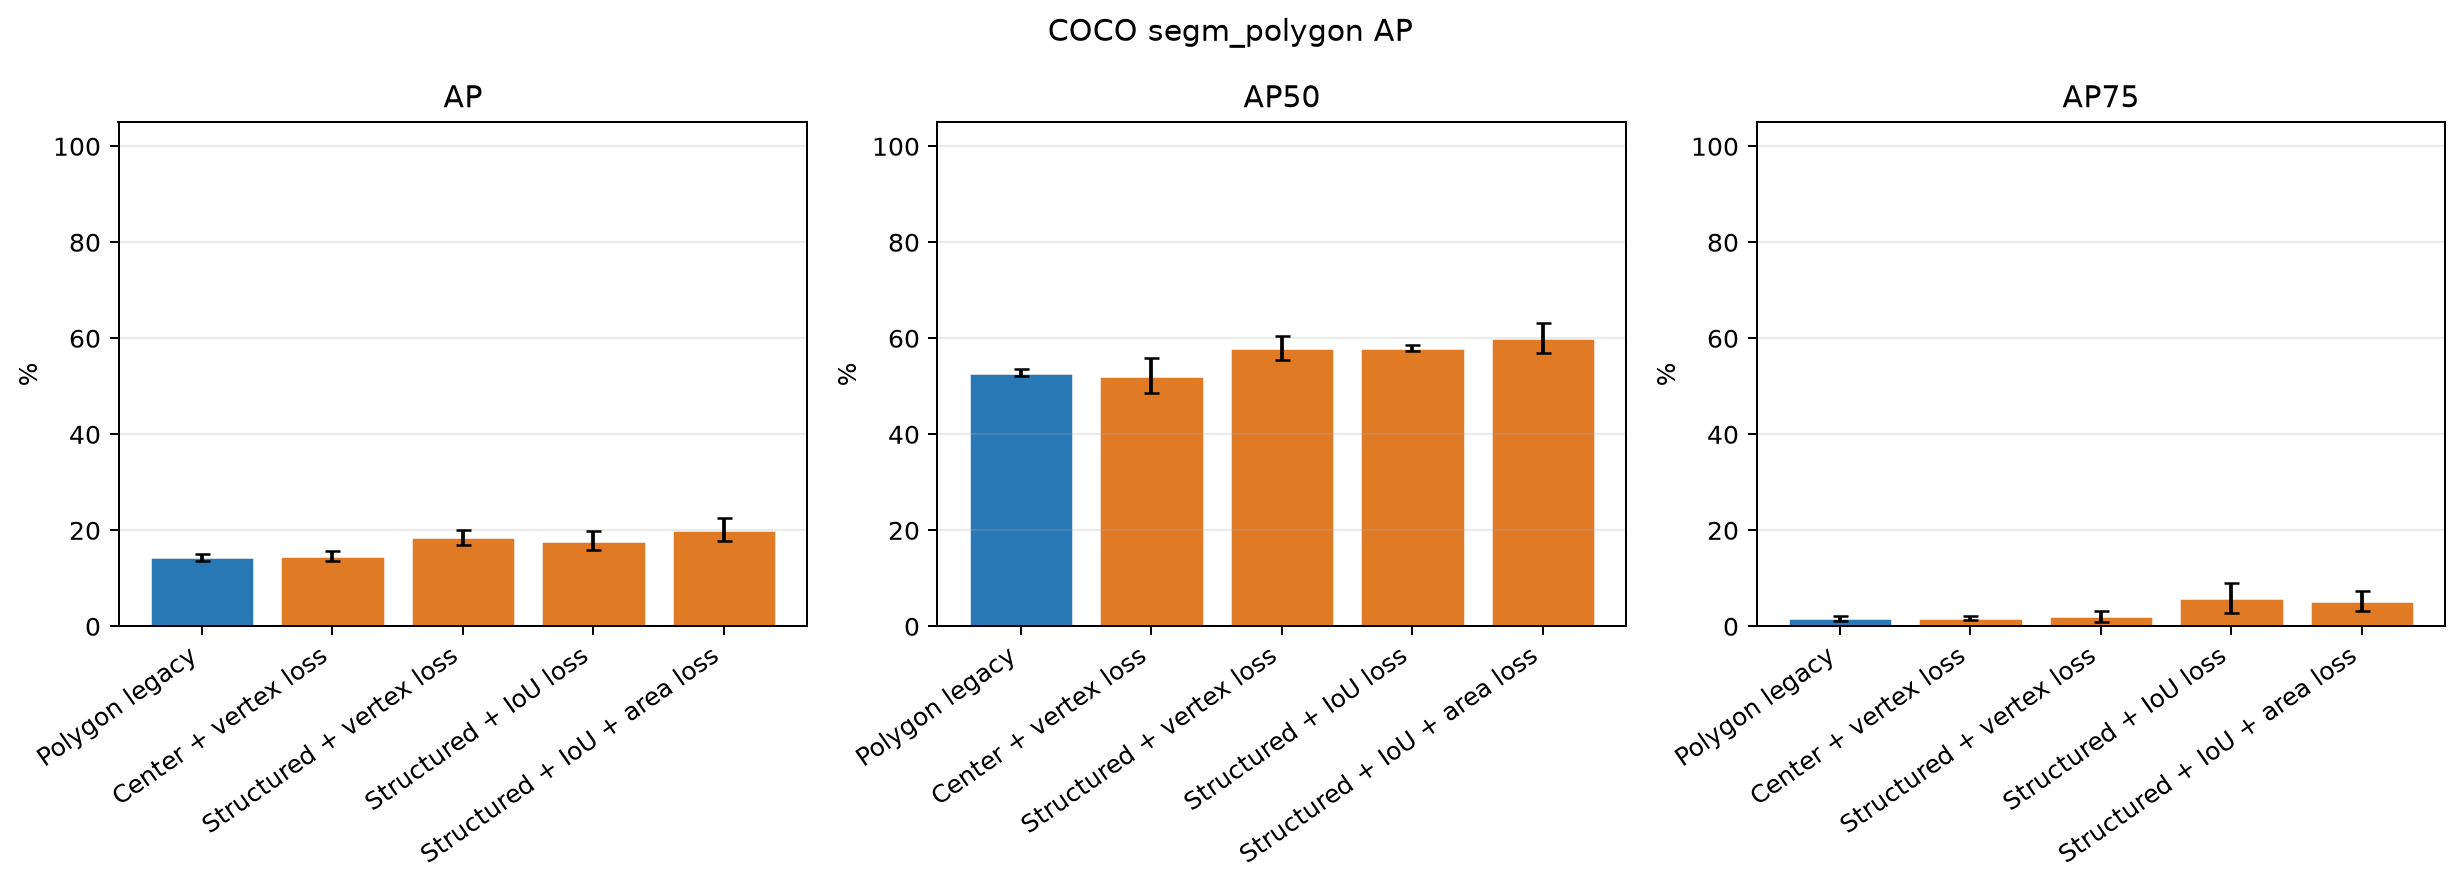
\includegraphics[width=0.8\linewidth]{reports/coco_ap_segm_polygon.png}
\caption{AP, AP50 e AP75 para as variantes poligonais atuais, agregadas em três
seeds.}
\label{fig:polygon_ablation_ap}
\end{figure}

\begin{figure}[H]
\centering
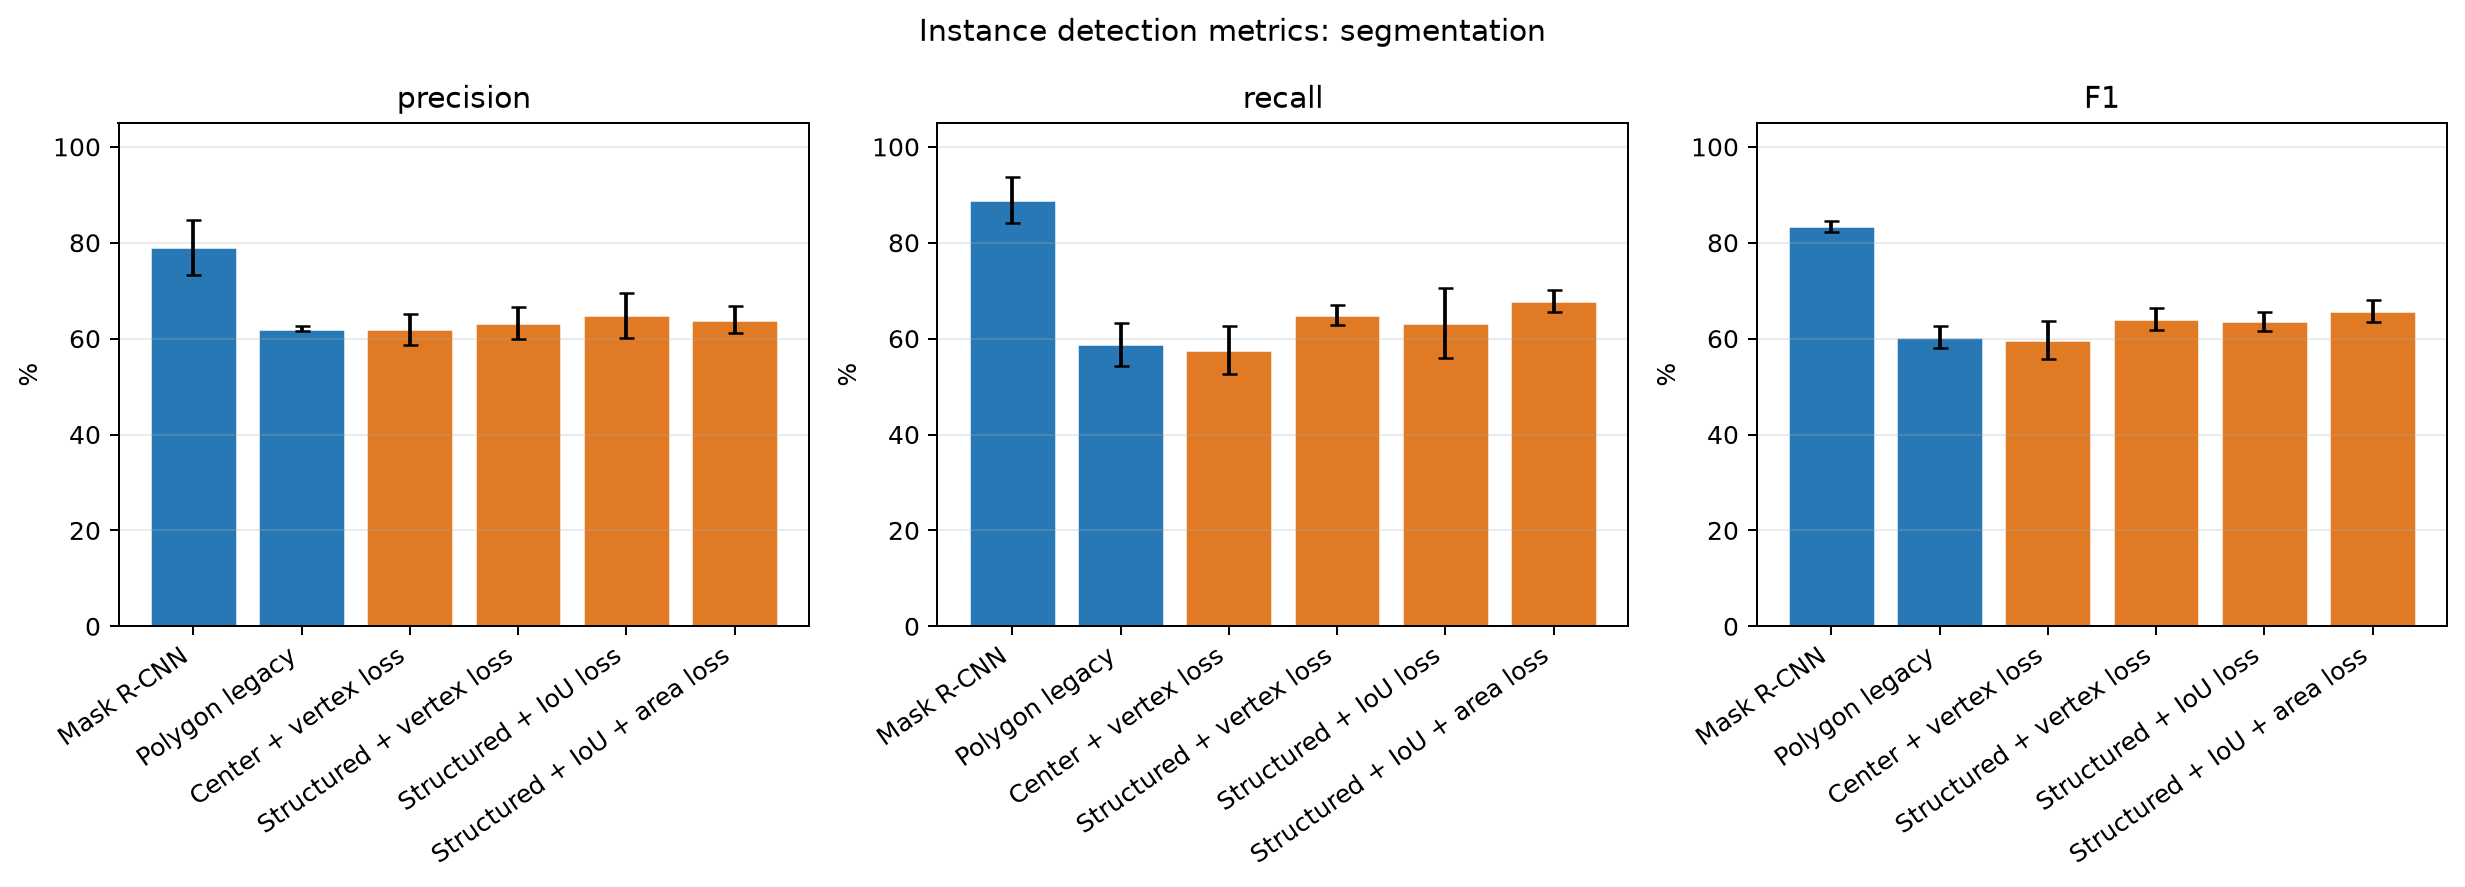
\includegraphics[width=0.8\linewidth]{reports/detection_metrics_segmentation.png}
\caption{Precisão, recall e F1 por instância para as saídas de máscara e
poligonais atuais. O limiar é escolhido na validação.}
\label{fig:polygon_ablation_prf1}
\end{figure}

\begin{figure}[H]
\centering
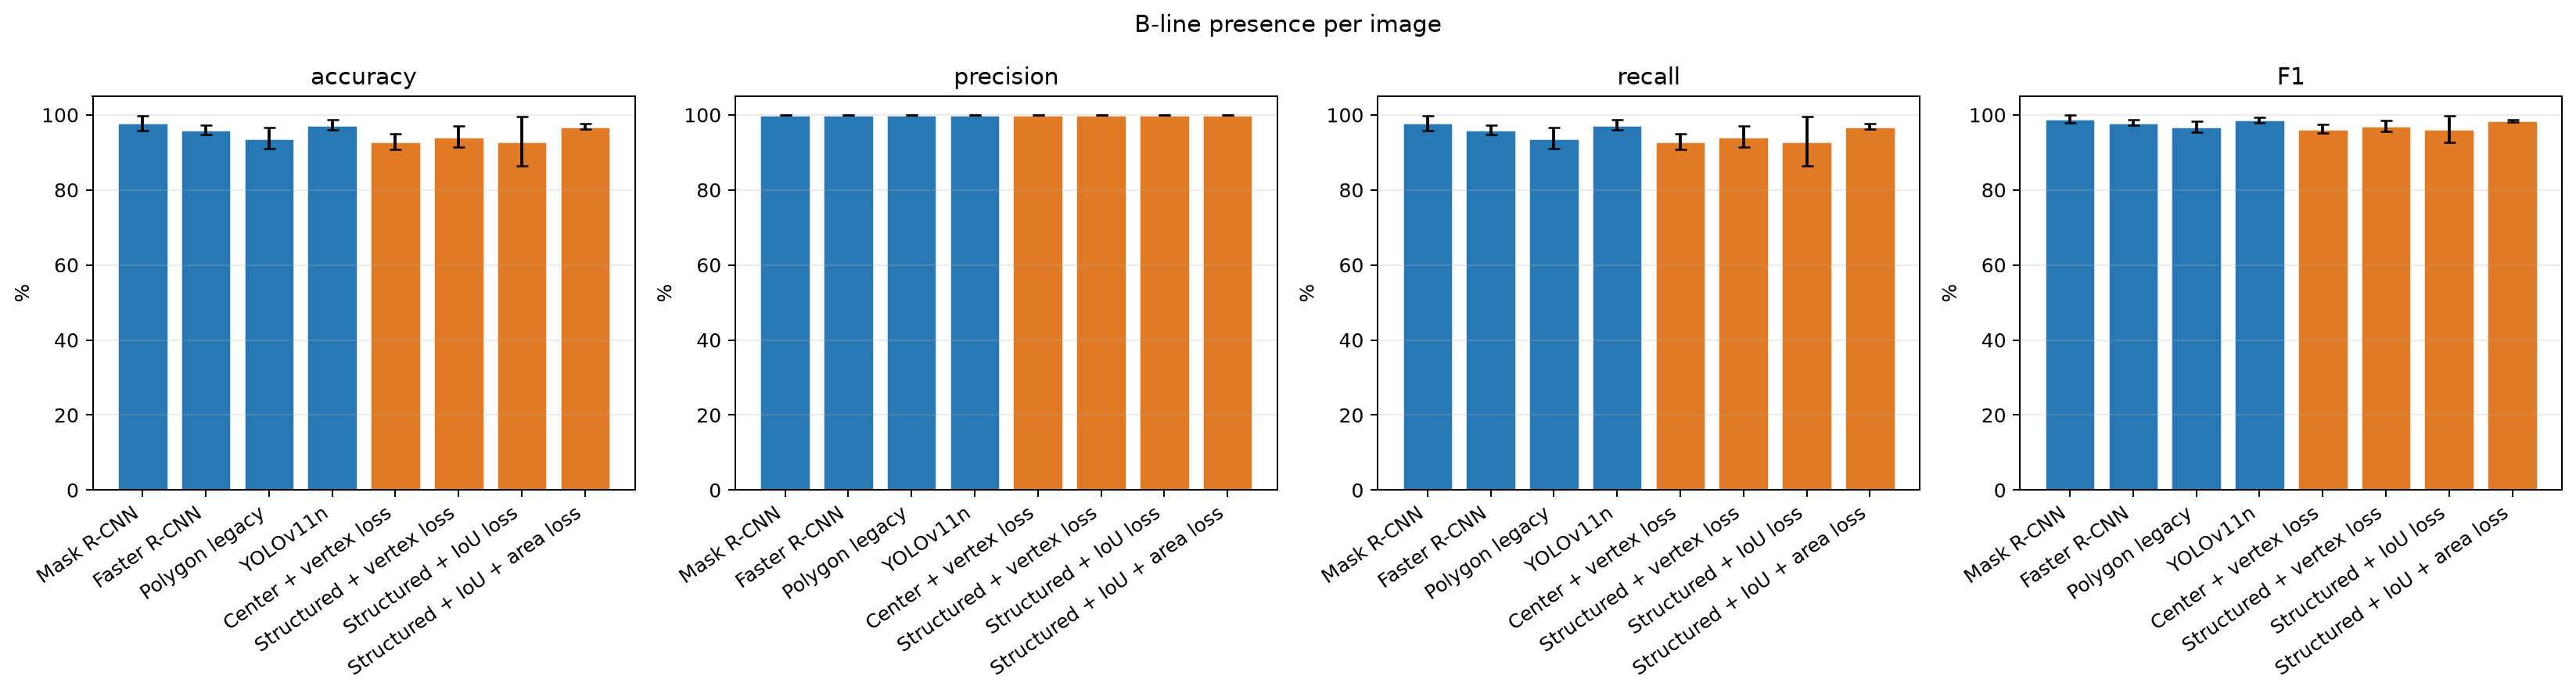
\includegraphics[width=0.8\linewidth]{reports/image_presence_metrics.png}
\caption{Métricas de presença por imagem para a rodada atual. Como não há imagens
negativas no split de validação, a figura não permite medir especificidade.}
\label{fig:image_presence}
\end{figure}

% ============================================================
\section{Resumo Geral}
\label{sec:resumo}
% ============================================================

\small
\setlength{\tabcolsep}{2pt}
\renewcommand{\arraystretch}{1.12}
\begin{longtable}{@{}p{3.5cm}p{6.0cm}p{6.0cm}@{}}
\caption{Comparação consolidada dos resultados anteriores preservados e da rodada
atual. Os valores estão em porcentagem. Para as configurações com três seeds, a
tabela mostra a média; as cinco configurações exploratórias de Polygon são
execuções únicas.}
\label{tab:resumo_comparativo}\\
\toprule
Modelo / configuração & AP / AP50 / AP75 & Precisão / recall / F1 por instância \\
\midrule
\endfirsthead
\multicolumn{3}{c}{\tablename\ \thetable{} --- continuação}\\
\toprule
Modelo / configuração & AP / AP50 / AP75 & Precisão / recall / F1 por instância \\
\midrule
\endhead
\midrule
\multicolumn{3}{r}{Continua na próxima página}\\
\endfoot
\bottomrule
\endlastfoot
Mask R-CNN, máscara & $42,88 / 86,14 / 35,98$ & $79,01 / 88,99 / 83,47$ \\
Mask R-CNN, caixa & $56,12 / 91,23 / 59,89$ & -- \\
Faster R-CNN, caixa & $52,37 / 87,95 / 55,05$ & $82,96 / 85,80 / 84,33$ \\
YOLOv11n, caixa & $55,86 / 85,26 / 59,39$ & $79,20 / 81,74 / 80,45$ \\
Polygon heatmap, resolução padrão & $15,0 / 37,1 / 11,9$ & $-- / -- / 49$ \\
Polygon heatmap, resolução dobrada & $3,8 / 10,8 / 2,7$ & $-- / -- / 25$ \\
Polygon regressão direta sem restrição & $12,2 / 54,2 / 1,4$ & $-- / 74 / 63$ \\
Polygon regressão com sigmoid & $4,3 / 22,9 / 0,1$ & $-- / 42 / 37$ \\
Polygon regressão com penalidade & $8,2 / 35,3 / 0,1$ & $-- / 55 / 46$ \\
Polygon regressão direta legacy & $14,36 / 52,86 / 1,63$ & $62,09 / 58,84 / 60,36$ \\
Polygon center-relative, vertex loss & $14,63 / 52,16 / 1,66$ & $61,98 / 57,68 / 59,71$ \\
Polygon structured, vertex loss & $18,57 / 57,98 / 2,08$ & $63,19 / 64,93 / 64,02$ \\
Polygon structured, IoU suave & $17,82 / 57,92 / 5,87$ & $64,86 / 63,19 / 63,64$ \\
Polygon structured, IoU + área & $20,15 / 60,08 / 5,26$ & $63,98 / 67,83 / 65,83$ \\
\end{longtable}

\normalsize
{\footnotesize
Em cada trio, a ordem é AP/AP50/AP75 ou precisão/recall/F1, conforme o cabeçalho.
As cinco primeiras configurações de Polygon são resultados exploratórios de
execução única; as cinco configurações poligonais seguintes são médias de três
seeds. O desvio-padrão amostral entre as três seeds foi omitido da tabela para
facilitar a leitura; portanto, ela mostra apenas as médias dos experimentos
repetidos. Os AP são de caixa para os detectores bbox, de máscara para Mask R-CNN
(máscara) e de região poligonal preenchida (\texttt{segm\_polygon}) para Polygon
Head; a avaliação usa COCOeval, mas as saídas máscara e polígono não são a mesma
representação. Nas configurações com três seeds, P/R/F1 usam IoU 0,50 e limiar
escolhido na validação. Nas linhas exploratórias, F1 e recall são os valores do
relatório anterior, sem recalcular precisão quando ela não foi reportada. O traço
indica métrica não registrada, não valor zero. Para Mask R-CNN, P/R/F1 foram
calculados para a saída de máscara; as métricas thresholdizadas da saída de caixa
não estão disponíveis nesta agregação.\par}

Os resultados atuais mostram que o AP de caixa dos baselines varia entre
$52,37\%$ e $56,12\%$. Para a Polygon Head, a representação estruturada com IoU e
área tem o maior AP médio atual ($20,15\%$) e F1 por instância ($65,83\%$), mas o
AP75 permanece baixo. A melhoria em relação à variante legacy é promissora, mas
descritiva: não demonstra significância estatística e não estabelece superioridade
em teste independente. O Mask R-CNN obtém AP de máscara $42,88\%$; como máscara
livre e polígono têm saídas distintas, essa diferença deve ser interpretada como
referência, não como comparação perfeitamente equivalente.

% ============================================================
\section{Limitações e Trabalhos Futuros}
\label{sec:limitacoes}
% ============================================================

\begin{itemize}
\item Os resultados da nova rodada usam três seeds por configuração e informam
média e desvio-padrão amostral. Ainda não foram calculados intervalos de confiança
pareados por imagem; as diferenças entre médias não demonstram, por si só,
significância estatística.

\item Na nova rodada, a seleção do checkpoint é alinhada à tarefa: bbox/AP para
Faster R-CNN, segm/AP para Mask R-CNN e segm\_polygon/AP para Polygon Head. Os
resultados exploratórios antigos de Polygon Head não têm logs completos para
confirmar a seleção de checkpoint usada naquela época.

\item O \textit{flip} horizontal foi desativado nas rodadas poligonais atuais.
O código agora oferece flip com reordenação canônica dos vértices, mas essa
variante não foi treinada. Mask R-CNN, Faster R-CNN e YOLO usam augmentations
próprias de seus pipelines; portanto, as famílias não compartilham um protocolo
de augmentations perfeitamente idêntico.

\item A métrica \texttt{segm\_polygon} não corresponde a uma AP de máscara por
pixel no sentido literal --- é o polígono avaliado pelo mesmo COCOeval de
segmentação, uma comparação justa, mas que deve ser identificada como tal.

\item Não existe, até o momento, um conjunto de teste anotado separado do de
validação.

\item A hipótese de caixas 12--16\% maiores veio de uma análise exploratória
anterior. A rotina de viés de bbox existe, mas ainda não foi executada nas
predições atuais; não se deve atribuir esse efeito a todos os detectores sem essa
medição.

\item A fonte dos exames, a unidade usada na separação dos splits e a eventual
separação por paciente não estão documentadas no repositório. Embora o total local
de 401 imagens coincida com o descrito para o LUS-BALD \cite{lusbald2025}, essa
coincidência não comprova a proveniência nem que as partições locais sejam as
publicadas. Também não estão documentados o número de anotadores nem medidas de
concordância entre eles.

\item Foram implementadas métricas geométricas (erro de vértices, IoU e área
poligonais, orientação, dimensões e taxa de polígonos inválidos) e categorias de
erro, mas os resultados não foram incluídos na agregação atual. O bootstrap
pareado por imagem também existe no código e ainda precisa ser executado. Essas
análises podem ser feitas a partir das predições salvas, sem repetir os treinos;
os comandos estão em \texttt{docs/REMOTE\_RUNBOOK.md}.

\item As métricas thresholdizadas e de presença são calculadas na validação. O
limiar de confiança foi escolhido para maximizar F1 nesse mesmo split. Além disso,
como todas as imagens de validação são positivas, métricas de presença não medem
especificidade nem desempenho em exames sem B-lines.

\item A loss de IoU suave é uma aproximação rasterizada de treinamento, não uma
loss analítica exata de interseção entre polígonos. Uma loss dedicada de fronteira
e a tarefa auxiliar de origem pleural não foram implementadas. As anotações atuais
não incluem pontos de origem pleural, então essa hipótese requer rótulos próprios.

\item \textbf{Escopo da literatura.} O desenho da Polygon Head foi motivado pela
engenharia do projeto e agora é contextualizado por métodos de detecção de
quadriláteros e objetos orientados
\cite{zhou2017east,liao2018textboxes,xu2020gliding,ding2019roi,law2018cornernet}.
Esses métodos não foram reproduzidos neste trabalho; a diferença de alvo e de
dataset impede tratá-los como comparações numéricas diretas. Uma revisão mais
ampla da literatura de B-Lines e localização pleural ainda é necessária para
justificar as escolhas de representação e priorizar novas ablações
\cite{lucassen2023,nabawanuka2025,abbasi2025}.
\end{itemize}

\begin{thebibliography}{99}
\bibitem{lin2014coco}
T.-Y. Lin et al., ``Microsoft COCO: Common Objects in Context,'' in
\textit{European Conference on Computer Vision (ECCV)}, 2014.
doi: \href{https://doi.org/10.1007/978-3-319-10602-1_48}{10.1007/978-3-319-10602-1\_48}.

\bibitem{he2017mask}
K. He, G. Gkioxari, P. Doll\'ar, and R. Girshick, ``Mask R-CNN,'' in
\textit{IEEE International Conference on Computer Vision (ICCV)}, 2017.
doi: \href{https://doi.org/10.1109/ICCV.2017.322}{10.1109/ICCV.2017.322}.

\bibitem{ren2015faster}
S. Ren, K. He, R. Girshick, and J. Sun, ``Faster R-CNN: Towards Real-Time Object
Detection with Region Proposal Networks,'' in \textit{Advances in Neural
Information Processing Systems}, 2015.

\bibitem{wu2019detectron2}
Y. Wu, A. Kirillov, F. Massa, W.-Y. Lo, and R. Girshick, ``Detectron2,'' software,
2019. \url{https://github.com/facebookresearch/detectron2}.

\bibitem{ultralytics2024}
Ultralytics, ``YOLO11,'' software documentation, 2024.
\url{https://docs.ultralytics.com/models/yolo11/}.

\bibitem{lucassen2023}
R. T. Lucassen et al., ``Deep Learning for Detection and Localization of B-Lines
in Lung Ultrasound,'' \textit{IEEE Journal of Biomedical and Health Informatics},
2023. \url{https://pmc.ncbi.nlm.nih.gov/articles/PMC10540221/}.

\bibitem{lusbald2025}
N. Okila et al., ``Lung Ultrasound Imaging Dataset for Accurate Detection
and Localization of LUS Vertical Artifact,'' \textit{Scientific Data}, 2025.
doi: \href{https://doi.org/10.1038/s41597-025-05854-4}{10.1038/s41597-025-05854-4}.

\bibitem{nabawanuka2025}
N. Okila et al., ``Deep Learning for Accurate B-Line Detection and
Localization in Lung Ultrasound Imaging,'' \textit{Frontiers in Artificial
Intelligence}, 2025. doi:
\href{https://doi.org/10.3389/frai.2025.1560523}{10.3389/frai.2025.1560523}.

\bibitem{abbasi2025}
S. Abbasi et al., ``Improved A-Line and B-Line Detection in Lung Ultrasound Using
Deep Learning with Boundary-Aware Dice Loss,'' \textit{Bioengineering}, vol. 12,
no. 3, 2025. doi:
\href{https://doi.org/10.3390/bioengineering12030311}{10.3390/bioengineering12030311}.

\bibitem{zhou2017east}
X. Zhou et al., ``EAST: An Efficient and Accurate Scene Text Detector,'' in
\textit{IEEE Conference on Computer Vision and Pattern Recognition (CVPR)}, 2017.

\bibitem{liao2018textboxes}
M. Liao, B. Shi, and X. Bai, ``TextBoxes++: A Single-Shot Oriented Scene Text
Detector,'' \textit{IEEE Transactions on Image Processing}, vol. 27, no. 8,
pp. 3676--3690, 2018. doi:
\href{https://doi.org/10.1109/TIP.2018.2825107}{10.1109/TIP.2018.2825107}.

\bibitem{xu2020gliding}
Y. Xu et al., ``Gliding Vertex on the Horizontal Bounding Box for Multi-Oriented
Object Detection,'' \textit{IEEE Transactions on Pattern Analysis and Machine
Intelligence}, 2020. doi:
\href{https://doi.org/10.1109/TPAMI.2020.2974745}{10.1109/TPAMI.2020.2974745}.

\bibitem{ding2019roi}
J. Ding, N. Xue, Y. Long, G.-S. Xia, and Q. Lu, ``Learning RoI Transformer for
Oriented Object Detection in Aerial Images,'' in \textit{IEEE/CVF Conference on
Computer Vision and Pattern Recognition (CVPR)}, 2019.

\bibitem{law2018cornernet}
H. Law and J. Deng, ``CornerNet: Detecting Objects as Paired Keypoints,'' in
\textit{European Conference on Computer Vision (ECCV)}, 2018.
\end{thebibliography}

\end{document}
